\documentclass[twoside]{book}

% Packages required by doxygen
\usepackage{fixltx2e}
\usepackage{calc}
\usepackage{doxygen}
\usepackage[export]{adjustbox} % also loads graphicx
\usepackage{graphicx}
\usepackage[utf8]{inputenc}
\usepackage{makeidx}
\usepackage{multicol}
\usepackage{multirow}
\PassOptionsToPackage{warn}{textcomp}
\usepackage{textcomp}
\usepackage[nointegrals]{wasysym}
\usepackage[table]{xcolor}

% Font selection
\usepackage[T1]{fontenc}
\usepackage[scaled=.90]{helvet}
\usepackage{courier}
\usepackage{amssymb}
\usepackage{sectsty}
\renewcommand{\familydefault}{\sfdefault}
\allsectionsfont{%
  \fontseries{bc}\selectfont%
  \color{darkgray}%
}
\renewcommand{\DoxyLabelFont}{%
  \fontseries{bc}\selectfont%
  \color{darkgray}%
}
\newcommand{\+}{\discretionary{\mbox{\scriptsize$\hookleftarrow$}}{}{}}

% Page & text layout
\usepackage{geometry}
\geometry{%
  a4paper,%
  top=2.5cm,%
  bottom=2.5cm,%
  left=2.5cm,%
  right=2.5cm%
}
\tolerance=750
\hfuzz=15pt
\hbadness=750
\setlength{\emergencystretch}{15pt}
\setlength{\parindent}{0cm}
\setlength{\parskip}{3ex plus 2ex minus 2ex}
\makeatletter
\renewcommand{\paragraph}{%
  \@startsection{paragraph}{4}{0ex}{-1.0ex}{1.0ex}{%
    \normalfont\normalsize\bfseries\SS@parafont%
  }%
}
\renewcommand{\subparagraph}{%
  \@startsection{subparagraph}{5}{0ex}{-1.0ex}{1.0ex}{%
    \normalfont\normalsize\bfseries\SS@subparafont%
  }%
}
\makeatother

% Headers & footers
\usepackage{fancyhdr}
\pagestyle{fancyplain}
\fancyhead[LE]{\fancyplain{}{\bfseries\thepage}}
\fancyhead[CE]{\fancyplain{}{}}
\fancyhead[RE]{\fancyplain{}{\bfseries\leftmark}}
\fancyhead[LO]{\fancyplain{}{\bfseries\rightmark}}
\fancyhead[CO]{\fancyplain{}{}}
\fancyhead[RO]{\fancyplain{}{\bfseries\thepage}}
\fancyfoot[LE]{\fancyplain{}{}}
\fancyfoot[CE]{\fancyplain{}{}}
\fancyfoot[RE]{\fancyplain{}{\bfseries\scriptsize Generated by Doxygen }}
\fancyfoot[LO]{\fancyplain{}{\bfseries\scriptsize Generated by Doxygen }}
\fancyfoot[CO]{\fancyplain{}{}}
\fancyfoot[RO]{\fancyplain{}{}}
\renewcommand{\footrulewidth}{0.4pt}
\renewcommand{\chaptermark}[1]{%
  \markboth{#1}{}%
}
\renewcommand{\sectionmark}[1]{%
  \markright{\thesection\ #1}%
}

% Indices & bibliography
\usepackage{natbib}
\usepackage[titles]{tocloft}
\setcounter{tocdepth}{3}
\setcounter{secnumdepth}{5}
\makeindex

% Hyperlinks (required, but should be loaded last)
\usepackage{ifpdf}
\ifpdf
  \usepackage[pdftex,pagebackref=true]{hyperref}
\else
  \usepackage[ps2pdf,pagebackref=true]{hyperref}
\fi
\hypersetup{%
  colorlinks=true,%
  linkcolor=blue,%
  citecolor=blue,%
  unicode%
}

% Custom commands
\newcommand{\clearemptydoublepage}{%
  \newpage{\pagestyle{empty}\cleardoublepage}%
}

\usepackage{caption}
\captionsetup{labelsep=space,justification=centering,font={bf},singlelinecheck=off,skip=4pt,position=top}

%===== C O N T E N T S =====

\begin{document}

% Titlepage & ToC
\hypersetup{pageanchor=false,
             bookmarksnumbered=true,
             pdfencoding=unicode
            }
\pagenumbering{alph}
\begin{titlepage}
\vspace*{7cm}
\begin{center}%
{\Large Graphs }\\
\vspace*{1cm}
{\large Generated by Doxygen 1.8.13}\\
\end{center}
\end{titlepage}
\clearemptydoublepage
\pagenumbering{roman}
\tableofcontents
\clearemptydoublepage
\pagenumbering{arabic}
\hypersetup{pageanchor=true}

%--- Begin generated contents ---
\chapter{Namespace Index}
\section{Packages}
Here are the packages with brief descriptions (if available)\+:\begin{DoxyCompactList}
\item\contentsline{section}{\hyperlink{namespace_graph}{Graph} }{\pageref{namespace_graph}}{}
\end{DoxyCompactList}

\chapter{Hierarchical Index}
\section{Class Hierarchy}
This inheritance list is sorted roughly, but not completely, alphabetically\+:\begin{DoxyCompactList}
\item \contentsline{section}{Graph.\+Edge}{\pageref{class_graph_1_1_edge}}{}
\item Exception\begin{DoxyCompactList}
\item \contentsline{section}{Graph.\+Algorithm.\+No\+Such\+Path\+Exception}{\pageref{class_graph_1_1_algorithm_1_1_no_such_path_exception}}{}
\end{DoxyCompactList}
\item Form\begin{DoxyCompactList}
\item \contentsline{section}{Graph.\+About\+Box1}{\pageref{class_graph_1_1_about_box1}}{}
\item \contentsline{section}{Graph.\+Edge\+Weight\+Dialog}{\pageref{class_graph_1_1_edge_weight_dialog}}{}
\item \contentsline{section}{Graph.\+Graph\+Name\+Dialog}{\pageref{class_graph_1_1_graph_name_dialog}}{}
\item \contentsline{section}{Graph.\+Main\+Window}{\pageref{class_graph_1_1_main_window}}{}
\item \contentsline{section}{Graph.\+New\+Vertex\+Dialog}{\pageref{class_graph_1_1_new_vertex_dialog}}{}
\end{DoxyCompactList}
\item \contentsline{section}{Graph.\+Graph}{\pageref{class_graph_1_1_graph}}{}
\item \contentsline{section}{Graph.\+Vertex}{\pageref{class_graph_1_1_vertex}}{}
\end{DoxyCompactList}

\chapter{Class Index}
\section{Class List}
Here are the classes, structs, unions and interfaces with brief descriptions\+:\begin{DoxyCompactList}
\item\contentsline{section}{\hyperlink{class_graph_1_1_about_box1}{Graph.\+About\+Box1} }{\pageref{class_graph_1_1_about_box1}}{}
\item\contentsline{section}{\hyperlink{class_graph_1_1_edge}{Graph.\+Edge} \\*A class that rappresents an edge in a graph }{\pageref{class_graph_1_1_edge}}{}
\item\contentsline{section}{\hyperlink{class_graph_1_1_edge_weight_dialog}{Graph.\+Edge\+Weight\+Dialog} }{\pageref{class_graph_1_1_edge_weight_dialog}}{}
\item\contentsline{section}{\hyperlink{class_graph_1_1_graph}{Graph.\+Graph} \\*A class that rappresents a graph }{\pageref{class_graph_1_1_graph}}{}
\item\contentsline{section}{\hyperlink{class_graph_1_1_graph_name_dialog}{Graph.\+Graph\+Name\+Dialog} }{\pageref{class_graph_1_1_graph_name_dialog}}{}
\item\contentsline{section}{\hyperlink{class_graph_1_1_main_window}{Graph.\+Main\+Window} \\*Main Window for the application }{\pageref{class_graph_1_1_main_window}}{}
\item\contentsline{section}{\hyperlink{class_graph_1_1_new_vertex_dialog}{Graph.\+New\+Vertex\+Dialog} }{\pageref{class_graph_1_1_new_vertex_dialog}}{}
\item\contentsline{section}{\hyperlink{class_graph_1_1_algorithm_1_1_no_such_path_exception}{Graph.\+Algorithm.\+No\+Such\+Path\+Exception} \\*An exception that is thrown when the path from A to B doesn\textquotesingle{}t exist }{\pageref{class_graph_1_1_algorithm_1_1_no_such_path_exception}}{}
\item\contentsline{section}{\hyperlink{class_graph_1_1_vertex}{Graph.\+Vertex} \\*A class that represents a vertex in a graph }{\pageref{class_graph_1_1_vertex}}{}
\end{DoxyCompactList}

\chapter{Namespace Documentation}
\hypertarget{namespace_graph}{}\section{Graph Namespace Reference}
\label{namespace_graph}\index{Graph@{Graph}}
\subsection*{Classes}
\begin{DoxyCompactItemize}
\item 
class \hyperlink{class_graph_1_1_about_box1}{About\+Box1}
\item 
class {\bfseries Algorithm}
\begin{DoxyCompactList}\small\item\em Static class that contains common algorithms on graphs \end{DoxyCompactList}\item 
class \hyperlink{class_graph_1_1_edge}{Edge}
\begin{DoxyCompactList}\small\item\em A class that rappresents an edge in a graph \end{DoxyCompactList}\item 
class \hyperlink{class_graph_1_1_edge_weight_dialog}{Edge\+Weight\+Dialog}
\item 
class \hyperlink{class_graph_1_1_graph}{Graph}
\begin{DoxyCompactList}\small\item\em A class that rappresents a graph \end{DoxyCompactList}\item 
class \hyperlink{class_graph_1_1_graph_name_dialog}{Graph\+Name\+Dialog}
\item 
class \hyperlink{class_graph_1_1_main_window}{Main\+Window}
\begin{DoxyCompactList}\small\item\em Main Window for the application \end{DoxyCompactList}\item 
class \hyperlink{class_graph_1_1_new_vertex_dialog}{New\+Vertex\+Dialog}
\item 
class \hyperlink{class_graph_1_1_vertex}{Vertex}
\begin{DoxyCompactList}\small\item\em A class that represents a vertex in a graph \end{DoxyCompactList}\end{DoxyCompactItemize}
\subsection*{Typedefs}
\begin{DoxyCompactItemize}
\item 
\mbox{\Hypertarget{namespace_graph_aaa1a0c11dafb790d64f39be3bff79717}\label{namespace_graph_aaa1a0c11dafb790d64f39be3bff79717}} 
using {\bfseries Dijkstra\+Result} = Tuple$<$ List$<$ \hyperlink{class_graph_1_1_vertex}{Vertex} $>$, int $>$
\end{DoxyCompactItemize}

\chapter{Class Documentation}
\hypertarget{class_graph_1_1_about_box1}{}\section{Graph.\+About\+Box1 Class Reference}
\label{class_graph_1_1_about_box1}\index{Graph.\+About\+Box1@{Graph.\+About\+Box1}}
Inheritance diagram for Graph.\+About\+Box1\+:\begin{figure}[H]
\begin{center}
\leavevmode
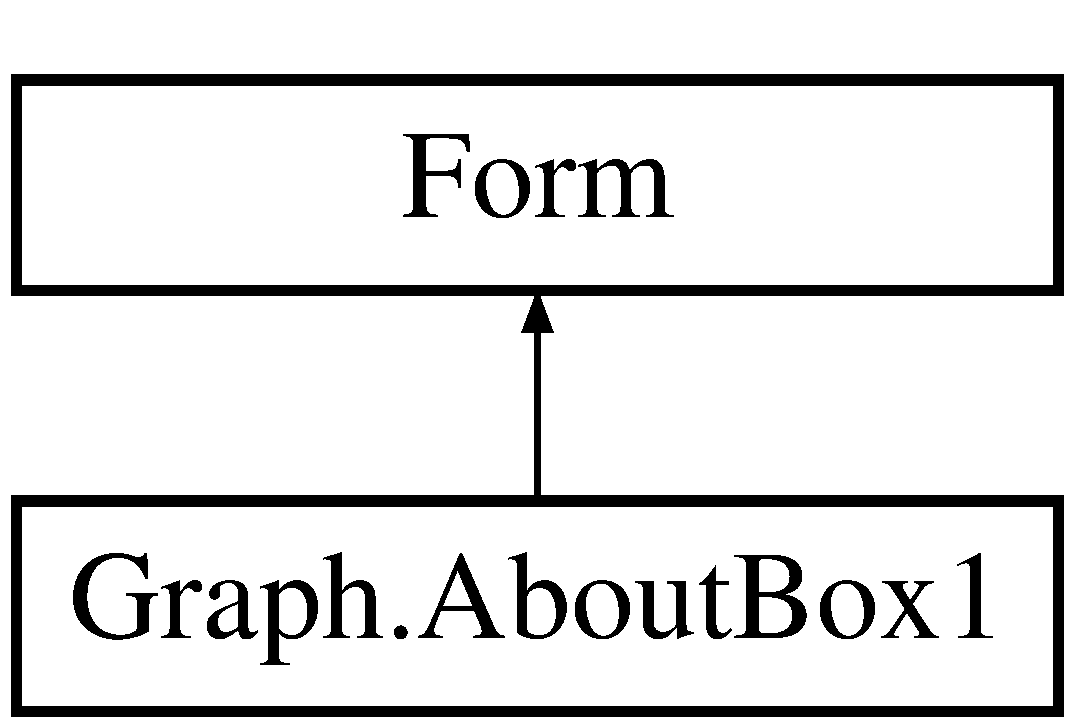
\includegraphics[height=2.000000cm]{class_graph_1_1_about_box1}
\end{center}
\end{figure}
\subsection*{Protected Member Functions}
\begin{DoxyCompactItemize}
\item 
override void \hyperlink{class_graph_1_1_about_box1_a972150c43ff56c63ca2172f781c56ec9}{Dispose} (bool disposing)
\begin{DoxyCompactList}\small\item\em Pulire le risorse in uso. \end{DoxyCompactList}\end{DoxyCompactItemize}
\subsection*{Properties}
\begin{DoxyCompactItemize}
\item 
\mbox{\Hypertarget{class_graph_1_1_about_box1_a975e47f83f7c0a14be043a0c3db7eb83}\label{class_graph_1_1_about_box1_a975e47f83f7c0a14be043a0c3db7eb83}} 
string {\bfseries Assembly\+Title}\hspace{0.3cm}{\ttfamily  \mbox{[}get\mbox{]}}
\item 
\mbox{\Hypertarget{class_graph_1_1_about_box1_a85ea56ecca02a69659dfd98edede7d67}\label{class_graph_1_1_about_box1_a85ea56ecca02a69659dfd98edede7d67}} 
string {\bfseries Assembly\+Version}\hspace{0.3cm}{\ttfamily  \mbox{[}get\mbox{]}}
\item 
\mbox{\Hypertarget{class_graph_1_1_about_box1_adca7c6ee8aec9435114a199409831e30}\label{class_graph_1_1_about_box1_adca7c6ee8aec9435114a199409831e30}} 
string {\bfseries Assembly\+Description}\hspace{0.3cm}{\ttfamily  \mbox{[}get\mbox{]}}
\item 
\mbox{\Hypertarget{class_graph_1_1_about_box1_a4c4fe84609ba9d173e6f76867ca153cf}\label{class_graph_1_1_about_box1_a4c4fe84609ba9d173e6f76867ca153cf}} 
string {\bfseries Assembly\+Product}\hspace{0.3cm}{\ttfamily  \mbox{[}get\mbox{]}}
\item 
\mbox{\Hypertarget{class_graph_1_1_about_box1_a729d1d2155be35569340f38121c71a8c}\label{class_graph_1_1_about_box1_a729d1d2155be35569340f38121c71a8c}} 
string {\bfseries Assembly\+Copyright}\hspace{0.3cm}{\ttfamily  \mbox{[}get\mbox{]}}
\item 
\mbox{\Hypertarget{class_graph_1_1_about_box1_a79dc9db943a090256db6f5ce96830332}\label{class_graph_1_1_about_box1_a79dc9db943a090256db6f5ce96830332}} 
string {\bfseries Assembly\+Company}\hspace{0.3cm}{\ttfamily  \mbox{[}get\mbox{]}}
\end{DoxyCompactItemize}


\subsection{Member Function Documentation}
\mbox{\Hypertarget{class_graph_1_1_about_box1_a972150c43ff56c63ca2172f781c56ec9}\label{class_graph_1_1_about_box1_a972150c43ff56c63ca2172f781c56ec9}} 
\index{Graph\+::\+About\+Box1@{Graph\+::\+About\+Box1}!Dispose@{Dispose}}
\index{Dispose@{Dispose}!Graph\+::\+About\+Box1@{Graph\+::\+About\+Box1}}
\subsubsection{\texorpdfstring{Dispose()}{Dispose()}}
{\footnotesize\ttfamily override void Graph.\+About\+Box1.\+Dispose (\begin{DoxyParamCaption}\item[{bool}]{disposing }\end{DoxyParamCaption})\hspace{0.3cm}{\ttfamily [protected]}}



Pulire le risorse in uso. 



The documentation for this class was generated from the following files\+:\begin{DoxyCompactItemize}
\item 
C\+:/\+Users/aless/\+One\+Drive/\+Documenti/\+Visual Studio 2017/\+Projects/\+Graph/\+Graph/About\+Box1.\+cs\item 
C\+:/\+Users/aless/\+One\+Drive/\+Documenti/\+Visual Studio 2017/\+Projects/\+Graph/\+Graph/About\+Box1.\+Designer.\+cs\end{DoxyCompactItemize}

\hypertarget{class_graph_1_1_edge}{}\section{Graph.\+Edge Class Reference}
\label{class_graph_1_1_edge}\index{Graph.\+Edge@{Graph.\+Edge}}


A class that rappresents an edge in a graph  


\subsection*{Public Member Functions}
\begin{DoxyCompactItemize}
\item 
\hyperlink{class_graph_1_1_edge_ada1a26604e35b231a38ac5ed2f7bc92f}{Edge} (\hyperlink{class_graph_1_1_vertex}{Vertex} from, \hyperlink{class_graph_1_1_vertex}{Vertex} to, int weight, bool bidirectional)
\begin{DoxyCompactList}\small\item\em Constructor of an edge \end{DoxyCompactList}\item 
override string \hyperlink{class_graph_1_1_edge_a21f9dcb22638dd0e38356bc81b35e219}{To\+String} ()
\begin{DoxyCompactList}\small\item\em Returns string rappresentation of the object \end{DoxyCompactList}\end{DoxyCompactItemize}
\subsection*{Properties}
\begin{DoxyCompactItemize}
\item 
\hyperlink{class_graph_1_1_vertex}{Vertex} \hyperlink{class_graph_1_1_edge_aa8c3fe4814c4db91276161e22eb8a930}{From}\hspace{0.3cm}{\ttfamily  \mbox{[}get\mbox{]}}
\begin{DoxyCompactList}\small\item\em \hyperlink{class_graph_1_1_vertex}{Vertex} where the edge starts \end{DoxyCompactList}\item 
\hyperlink{class_graph_1_1_vertex}{Vertex} \hyperlink{class_graph_1_1_edge_a55661e4bd903eb6d33e48129124360e8}{To}\hspace{0.3cm}{\ttfamily  \mbox{[}get\mbox{]}}
\begin{DoxyCompactList}\small\item\em \hyperlink{class_graph_1_1_vertex}{Vertex} that the edge connects to \end{DoxyCompactList}\item 
bool \hyperlink{class_graph_1_1_edge_a01a68bb38bf2ea3498d9ff9be3b74338}{Color}\hspace{0.3cm}{\ttfamily  \mbox{[}get, set\mbox{]}}
\begin{DoxyCompactList}\small\item\em Color of the edge -\/ true = red, false = black \end{DoxyCompactList}\item 
int \hyperlink{class_graph_1_1_edge_a34f6965d86e366584d5679bba8fe54ad}{Weight}\hspace{0.3cm}{\ttfamily  \mbox{[}get, set\mbox{]}}
\begin{DoxyCompactList}\small\item\em Weight of the edge \end{DoxyCompactList}\item 
bool \hyperlink{class_graph_1_1_edge_a26fcbf19716fd9202a8e995b305fad17}{Bidirectional}\hspace{0.3cm}{\ttfamily  \mbox{[}get, set\mbox{]}}
\begin{DoxyCompactList}\small\item\em true if the edge is bidirectional \end{DoxyCompactList}\end{DoxyCompactItemize}


\subsection{Detailed Description}
A class that rappresents an edge in a graph 



\subsection{Constructor \& Destructor Documentation}
\mbox{\Hypertarget{class_graph_1_1_edge_ada1a26604e35b231a38ac5ed2f7bc92f}\label{class_graph_1_1_edge_ada1a26604e35b231a38ac5ed2f7bc92f}} 
\index{Graph\+::\+Edge@{Graph\+::\+Edge}!Edge@{Edge}}
\index{Edge@{Edge}!Graph\+::\+Edge@{Graph\+::\+Edge}}
\subsubsection{\texorpdfstring{Edge()}{Edge()}}
{\footnotesize\ttfamily Graph.\+Edge.\+Edge (\begin{DoxyParamCaption}\item[{\hyperlink{class_graph_1_1_vertex}{Vertex}}]{from,  }\item[{\hyperlink{class_graph_1_1_vertex}{Vertex}}]{to,  }\item[{int}]{weight,  }\item[{bool}]{bidirectional }\end{DoxyParamCaption})}



Constructor of an edge 


\begin{DoxyParams}{Parameters}
{\em from} & vertex to connect from\\
\hline
{\em to} & vertex to connect to\\
\hline
{\em weight} & weight of the edge\\
\hline
{\em bidirectional} & true if bidirectional\\
\hline
\end{DoxyParams}


\subsection{Member Function Documentation}
\mbox{\Hypertarget{class_graph_1_1_edge_a21f9dcb22638dd0e38356bc81b35e219}\label{class_graph_1_1_edge_a21f9dcb22638dd0e38356bc81b35e219}} 
\index{Graph\+::\+Edge@{Graph\+::\+Edge}!To\+String@{To\+String}}
\index{To\+String@{To\+String}!Graph\+::\+Edge@{Graph\+::\+Edge}}
\subsubsection{\texorpdfstring{To\+String()}{ToString()}}
{\footnotesize\ttfamily override string Graph.\+Edge.\+To\+String (\begin{DoxyParamCaption}{ }\end{DoxyParamCaption})}



Returns string rappresentation of the object 

\begin{DoxyReturn}{Returns}
string rappresentation of the object
\end{DoxyReturn}


\subsection{Property Documentation}
\mbox{\Hypertarget{class_graph_1_1_edge_a26fcbf19716fd9202a8e995b305fad17}\label{class_graph_1_1_edge_a26fcbf19716fd9202a8e995b305fad17}} 
\index{Graph\+::\+Edge@{Graph\+::\+Edge}!Bidirectional@{Bidirectional}}
\index{Bidirectional@{Bidirectional}!Graph\+::\+Edge@{Graph\+::\+Edge}}
\subsubsection{\texorpdfstring{Bidirectional}{Bidirectional}}
{\footnotesize\ttfamily bool Graph.\+Edge.\+Bidirectional\hspace{0.3cm}{\ttfamily [get]}, {\ttfamily [set]}}



true if the edge is bidirectional 

\mbox{\Hypertarget{class_graph_1_1_edge_a01a68bb38bf2ea3498d9ff9be3b74338}\label{class_graph_1_1_edge_a01a68bb38bf2ea3498d9ff9be3b74338}} 
\index{Graph\+::\+Edge@{Graph\+::\+Edge}!Color@{Color}}
\index{Color@{Color}!Graph\+::\+Edge@{Graph\+::\+Edge}}
\subsubsection{\texorpdfstring{Color}{Color}}
{\footnotesize\ttfamily bool Graph.\+Edge.\+Color\hspace{0.3cm}{\ttfamily [get]}, {\ttfamily [set]}}



Color of the edge -\/ true = red, false = black 

\mbox{\Hypertarget{class_graph_1_1_edge_aa8c3fe4814c4db91276161e22eb8a930}\label{class_graph_1_1_edge_aa8c3fe4814c4db91276161e22eb8a930}} 
\index{Graph\+::\+Edge@{Graph\+::\+Edge}!From@{From}}
\index{From@{From}!Graph\+::\+Edge@{Graph\+::\+Edge}}
\subsubsection{\texorpdfstring{From}{From}}
{\footnotesize\ttfamily \hyperlink{class_graph_1_1_vertex}{Vertex} Graph.\+Edge.\+From\hspace{0.3cm}{\ttfamily [get]}}



\hyperlink{class_graph_1_1_vertex}{Vertex} where the edge starts 

\mbox{\Hypertarget{class_graph_1_1_edge_a55661e4bd903eb6d33e48129124360e8}\label{class_graph_1_1_edge_a55661e4bd903eb6d33e48129124360e8}} 
\index{Graph\+::\+Edge@{Graph\+::\+Edge}!To@{To}}
\index{To@{To}!Graph\+::\+Edge@{Graph\+::\+Edge}}
\subsubsection{\texorpdfstring{To}{To}}
{\footnotesize\ttfamily \hyperlink{class_graph_1_1_vertex}{Vertex} Graph.\+Edge.\+To\hspace{0.3cm}{\ttfamily [get]}}



\hyperlink{class_graph_1_1_vertex}{Vertex} that the edge connects to 

\mbox{\Hypertarget{class_graph_1_1_edge_a34f6965d86e366584d5679bba8fe54ad}\label{class_graph_1_1_edge_a34f6965d86e366584d5679bba8fe54ad}} 
\index{Graph\+::\+Edge@{Graph\+::\+Edge}!Weight@{Weight}}
\index{Weight@{Weight}!Graph\+::\+Edge@{Graph\+::\+Edge}}
\subsubsection{\texorpdfstring{Weight}{Weight}}
{\footnotesize\ttfamily int Graph.\+Edge.\+Weight\hspace{0.3cm}{\ttfamily [get]}, {\ttfamily [set]}}



Weight of the edge 



The documentation for this class was generated from the following file\+:\begin{DoxyCompactItemize}
\item 
C\+:/\+Users/aless/\+One\+Drive/\+Documenti/\+Visual Studio 2017/\+Projects/\+Graph/\+Graph/Edge.\+cs\end{DoxyCompactItemize}

\hypertarget{class_graph_1_1_edge_weight_dialog}{}\section{Graph.\+Edge\+Weight\+Dialog Class Reference}
\label{class_graph_1_1_edge_weight_dialog}\index{Graph.\+Edge\+Weight\+Dialog@{Graph.\+Edge\+Weight\+Dialog}}
Inheritance diagram for Graph.\+Edge\+Weight\+Dialog\+:\begin{figure}[H]
\begin{center}
\leavevmode
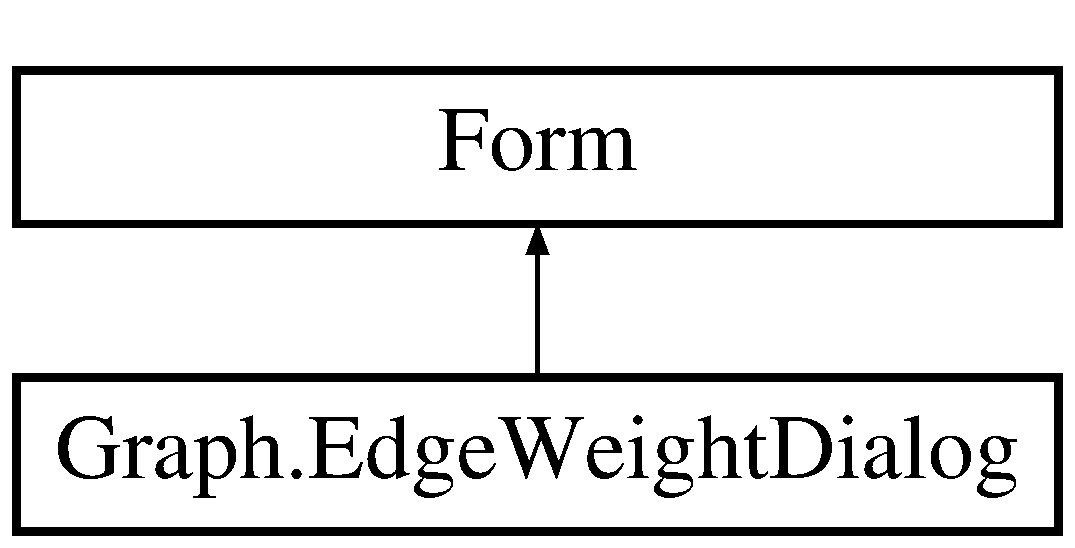
\includegraphics[height=2.000000cm]{class_graph_1_1_edge_weight_dialog}
\end{center}
\end{figure}
\subsection*{Public Member Functions}
\begin{DoxyCompactItemize}
\item 
\mbox{\Hypertarget{class_graph_1_1_edge_weight_dialog_a4502237ec4bf0376c452ad108ffe27d0}\label{class_graph_1_1_edge_weight_dialog_a4502237ec4bf0376c452ad108ffe27d0}} 
{\bfseries Edge\+Weight\+Dialog} (\hyperlink{class_graph_1_1_edge}{Edge} e)
\end{DoxyCompactItemize}
\subsection*{Protected Member Functions}
\begin{DoxyCompactItemize}
\item 
override void \hyperlink{class_graph_1_1_edge_weight_dialog_a861196924b6ecb2c9203005c4b73e27c}{Dispose} (bool disposing)
\begin{DoxyCompactList}\small\item\em Clean up any resources being used. \end{DoxyCompactList}\end{DoxyCompactItemize}
\subsection*{Properties}
\begin{DoxyCompactItemize}
\item 
\mbox{\Hypertarget{class_graph_1_1_edge_weight_dialog_ab7ca80d419f13a2881f8067b36d3d8b8}\label{class_graph_1_1_edge_weight_dialog_ab7ca80d419f13a2881f8067b36d3d8b8}} 
int {\bfseries Weight}\hspace{0.3cm}{\ttfamily  \mbox{[}get\mbox{]}}
\item 
\mbox{\Hypertarget{class_graph_1_1_edge_weight_dialog_ab16d01f448d9533fb43f0a9c0c19f603}\label{class_graph_1_1_edge_weight_dialog_ab16d01f448d9533fb43f0a9c0c19f603}} 
bool {\bfseries Bidirectional}\hspace{0.3cm}{\ttfamily  \mbox{[}get\mbox{]}}
\end{DoxyCompactItemize}


\subsection{Member Function Documentation}
\mbox{\Hypertarget{class_graph_1_1_edge_weight_dialog_a861196924b6ecb2c9203005c4b73e27c}\label{class_graph_1_1_edge_weight_dialog_a861196924b6ecb2c9203005c4b73e27c}} 
\index{Graph\+::\+Edge\+Weight\+Dialog@{Graph\+::\+Edge\+Weight\+Dialog}!Dispose@{Dispose}}
\index{Dispose@{Dispose}!Graph\+::\+Edge\+Weight\+Dialog@{Graph\+::\+Edge\+Weight\+Dialog}}
\subsubsection{\texorpdfstring{Dispose()}{Dispose()}}
{\footnotesize\ttfamily override void Graph.\+Edge\+Weight\+Dialog.\+Dispose (\begin{DoxyParamCaption}\item[{bool}]{disposing }\end{DoxyParamCaption})\hspace{0.3cm}{\ttfamily [protected]}}



Clean up any resources being used. 


\begin{DoxyParams}{Parameters}
{\em disposing} & true if managed resources should be disposed; otherwise, false.\\
\hline
\end{DoxyParams}


The documentation for this class was generated from the following files\+:\begin{DoxyCompactItemize}
\item 
C\+:/\+Users/aless/\+One\+Drive/\+Documenti/\+Visual Studio 2017/\+Projects/\+Graph/\+Graph/Edge\+Weight\+Dialog.\+cs\item 
C\+:/\+Users/aless/\+One\+Drive/\+Documenti/\+Visual Studio 2017/\+Projects/\+Graph/\+Graph/Edge\+Weight\+Dialog.\+Designer.\+cs\end{DoxyCompactItemize}

\hypertarget{class_graph_1_1_graph}{}\section{Graph.\+Graph Class Reference}
\label{class_graph_1_1_graph}\index{Graph.\+Graph@{Graph.\+Graph}}


A class that rappresents a graph  


\subsection*{Public Member Functions}
\begin{DoxyCompactItemize}
\item 
\mbox{\Hypertarget{class_graph_1_1_graph_a5eaf7b1db5e23c8de15f5d3d5cc2ff54}\label{class_graph_1_1_graph_a5eaf7b1db5e23c8de15f5d3d5cc2ff54}} 
bool {\bfseries Contains} (string name)
\item 
\hyperlink{class_graph_1_1_graph_a30ae09ae4861f50e9e2b52d4e5628335}{Graph} (string name)
\begin{DoxyCompactList}\small\item\em Constructs a new graph object \end{DoxyCompactList}\item 
int \hyperlink{class_graph_1_1_graph_a1340be74165a617b2229a1ddb6acb9d2}{Grade} ()
\begin{DoxyCompactList}\small\item\em Calculates total grade (number of edges) of the graph \end{DoxyCompactList}\item 
bool \hyperlink{class_graph_1_1_graph_a7704d6b3b279e38356b1a3a75f1b4b92}{Is\+Oriented} ()
\begin{DoxyCompactList}\small\item\em Checks if the graph is oriented or not \end{DoxyCompactList}\item 
virtual void \hyperlink{class_graph_1_1_graph_aac26679440a896ed404021c777070345}{Add\+Vertex} (\hyperlink{class_graph_1_1_vertex}{Vertex} vertex)
\begin{DoxyCompactList}\small\item\em Adds the a vertex to the graph \end{DoxyCompactList}\item 
void \hyperlink{class_graph_1_1_graph_af597a3c28572462384f64ea244e41db6}{Add\+Edge} (\hyperlink{class_graph_1_1_vertex}{Vertex} from, \hyperlink{class_graph_1_1_vertex}{Vertex} to, int weight, bool bidirectional=true)
\begin{DoxyCompactList}\small\item\em Adds an edge to the graph \end{DoxyCompactList}\item 
virtual void \hyperlink{class_graph_1_1_graph_a0b49bbae104d612158d6bbef9083d453}{Remove\+Edge} (\hyperlink{class_graph_1_1_edge}{Edge} edge)
\begin{DoxyCompactList}\small\item\em Removes an edge from the graph \end{DoxyCompactList}\item 
\hyperlink{class_graph_1_1_vertex}{Vertex} \hyperlink{class_graph_1_1_graph_ac68594326ba5c47cc44b0130bba6f924}{Get\+Or\+Create} (string name)
\begin{DoxyCompactList}\small\item\em If the vertex is already in the graph, it returns it. If not, create a new vertex, add it to the graph and returns it \end{DoxyCompactList}\item 
I\+Enumerator \hyperlink{class_graph_1_1_graph_a2588304efcfecc95d96afc3788a0288b}{Get\+Enumerator} ()
\begin{DoxyCompactList}\small\item\em Iterators that iterates on the Vertices\+Position of the graph \end{DoxyCompactList}\item 
override string \hyperlink{class_graph_1_1_graph_a156e417443003071243e2a22ba0a1533}{To\+String} ()
\begin{DoxyCompactList}\small\item\em Returns a string rappresentation of the graph. General informations such name, number of Vertices\+Position, grade are shown, with the list of Vertices\+Position and edges \end{DoxyCompactList}\item 
void \hyperlink{class_graph_1_1_graph_a0c9eb0d791d58368f214cbb96ac2a320}{Delete\+Vertex} (\hyperlink{class_graph_1_1_vertex}{Vertex} v)
\begin{DoxyCompactList}\small\item\em Remove a vertex from the graph, and the associated edges \end{DoxyCompactList}\item 
void \hyperlink{class_graph_1_1_graph_a4c16783a84526b65e8447f7061b38140}{Randomize\+Weights} ()
\begin{DoxyCompactList}\small\item\em Resets all the weights with random values in range 1..20 \end{DoxyCompactList}\item 
void \hyperlink{class_graph_1_1_graph_a04383a2aa3ff3f112d7b87408d7d573e}{Draw} (Graphics g)
\begin{DoxyCompactList}\small\item\em Draws the graph \end{DoxyCompactList}\item 
void \hyperlink{class_graph_1_1_graph_a74876b10cb94ff9f17ef17c674cc14d2}{Reset\+Colors} ()
\begin{DoxyCompactList}\small\item\em Resets the color of the graph \end{DoxyCompactList}\item 
\hyperlink{class_graph_1_1_vertex}{Vertex} \hyperlink{class_graph_1_1_graph_a3916416db4cf90b2afee5e7162c29875}{Vertex\+On\+Point} (int x, int y)
\begin{DoxyCompactList}\small\item\em Returns a vertex on the givern position, if it exists \end{DoxyCompactList}\item 
\hyperlink{class_graph_1_1_edge}{Edge} \hyperlink{class_graph_1_1_graph_ade3b10eb74bb3a2c8b1cbbe0069adfca}{Edge\+On\+Position} (int x, int y)
\begin{DoxyCompactList}\small\item\em Returns an edge near the specified position \end{DoxyCompactList}\item 
void \hyperlink{class_graph_1_1_graph_af328fc96d21cc0b8edba5ae71317b7e9}{Color\+List\+Of\+Vertices} (List$<$ \hyperlink{class_graph_1_1_vertex}{Vertex} $>$ vertices)
\begin{DoxyCompactList}\small\item\em Sets the color of a list of vertices and the edge between them red \end{DoxyCompactList}\item 
void \hyperlink{class_graph_1_1_graph_a7046489eb0f0149305bd361dd84c34a1}{Save\+Graph\+To\+File} (string file\+Name)
\begin{DoxyCompactList}\small\item\em Saves the current graph to file \end{DoxyCompactList}\end{DoxyCompactItemize}
\subsection*{Static Public Member Functions}
\begin{DoxyCompactItemize}
\item 
static \hyperlink{class_graph_1_1_graph}{Graph} \hyperlink{class_graph_1_1_graph_a7454bf91b0c01f5702082d5aa511c539}{From\+File} (string file\+Name)
\begin{DoxyCompactList}\small\item\em Imports a graph from a file \end{DoxyCompactList}\end{DoxyCompactItemize}
\subsection*{Public Attributes}
\begin{DoxyCompactItemize}
\item 
bool \hyperlink{class_graph_1_1_graph_a0daa42ad862bce4e14dca2652b565dc9}{Changed\+Since\+Last\+Save} =$>$ old\+Code != \hyperlink{class_graph_1_1_graph_a156e417443003071243e2a22ba0a1533}{To\+String}().Get\+Hash\+Code()
\begin{DoxyCompactList}\small\item\em Checks if the graph has changed since last save (works 99.\+9\% of the times!) \end{DoxyCompactList}\end{DoxyCompactItemize}
\subsection*{Properties}
\begin{DoxyCompactItemize}
\item 
string \hyperlink{class_graph_1_1_graph_a2635cdb256ccefb545cf402bd52a3f80}{Name}\hspace{0.3cm}{\ttfamily  \mbox{[}get, set\mbox{]}}
\begin{DoxyCompactList}\small\item\em Name of the graph \end{DoxyCompactList}\item 
static Size \hyperlink{class_graph_1_1_graph_ace6128caf64c731423b0ccd106f3ada6}{Size}\hspace{0.3cm}{\ttfamily  \mbox{[}get\mbox{]}}
\begin{DoxyCompactList}\small\item\em Size of the graph image \end{DoxyCompactList}\end{DoxyCompactItemize}


\subsection{Detailed Description}
A class that rappresents a graph 



\subsection{Constructor \& Destructor Documentation}
\mbox{\Hypertarget{class_graph_1_1_graph_a30ae09ae4861f50e9e2b52d4e5628335}\label{class_graph_1_1_graph_a30ae09ae4861f50e9e2b52d4e5628335}} 
\index{Graph\+::\+Graph@{Graph\+::\+Graph}!Graph@{Graph}}
\index{Graph@{Graph}!Graph\+::\+Graph@{Graph\+::\+Graph}}
\subsubsection{\texorpdfstring{Graph()}{Graph()}}
{\footnotesize\ttfamily Graph.\+Graph.\+Graph (\begin{DoxyParamCaption}\item[{string}]{name }\end{DoxyParamCaption})}



Constructs a new graph object 


\begin{DoxyParams}{Parameters}
{\em name} & name of the graph\\
\hline
\end{DoxyParams}


\subsection{Member Function Documentation}
\mbox{\Hypertarget{class_graph_1_1_graph_af597a3c28572462384f64ea244e41db6}\label{class_graph_1_1_graph_af597a3c28572462384f64ea244e41db6}} 
\index{Graph\+::\+Graph@{Graph\+::\+Graph}!Add\+Edge@{Add\+Edge}}
\index{Add\+Edge@{Add\+Edge}!Graph\+::\+Graph@{Graph\+::\+Graph}}
\subsubsection{\texorpdfstring{Add\+Edge()}{AddEdge()}}
{\footnotesize\ttfamily void Graph.\+Graph.\+Add\+Edge (\begin{DoxyParamCaption}\item[{\hyperlink{class_graph_1_1_vertex}{Vertex}}]{from,  }\item[{\hyperlink{class_graph_1_1_vertex}{Vertex}}]{to,  }\item[{int}]{weight,  }\item[{bool}]{bidirectional = {\ttfamily true} }\end{DoxyParamCaption})}



Adds an edge to the graph 


\begin{DoxyParams}{Parameters}
{\em from} & \hyperlink{class_graph_1_1_vertex}{Vertex} to start from\\
\hline
{\em to} & \hyperlink{class_graph_1_1_vertex}{Vertex} to connect to\\
\hline
{\em weight} & weight of the edge\\
\hline
{\em bidirectional} & true if the edge is bidirectional\\
\hline
\end{DoxyParams}

\begin{DoxyExceptions}{Exceptions}
{\em Exception} & from or to doesn\textquotesingle{}t exist in this graph\\
\hline
\end{DoxyExceptions}
\mbox{\Hypertarget{class_graph_1_1_graph_aac26679440a896ed404021c777070345}\label{class_graph_1_1_graph_aac26679440a896ed404021c777070345}} 
\index{Graph\+::\+Graph@{Graph\+::\+Graph}!Add\+Vertex@{Add\+Vertex}}
\index{Add\+Vertex@{Add\+Vertex}!Graph\+::\+Graph@{Graph\+::\+Graph}}
\subsubsection{\texorpdfstring{Add\+Vertex()}{AddVertex()}}
{\footnotesize\ttfamily virtual void Graph.\+Graph.\+Add\+Vertex (\begin{DoxyParamCaption}\item[{\hyperlink{class_graph_1_1_vertex}{Vertex}}]{vertex }\end{DoxyParamCaption})\hspace{0.3cm}{\ttfamily [virtual]}}



Adds the a vertex to the graph 


\begin{DoxyParams}{Parameters}
{\em vertex} & the vertex to add\\
\hline
\end{DoxyParams}
\mbox{\Hypertarget{class_graph_1_1_graph_af328fc96d21cc0b8edba5ae71317b7e9}\label{class_graph_1_1_graph_af328fc96d21cc0b8edba5ae71317b7e9}} 
\index{Graph\+::\+Graph@{Graph\+::\+Graph}!Color\+List\+Of\+Vertices@{Color\+List\+Of\+Vertices}}
\index{Color\+List\+Of\+Vertices@{Color\+List\+Of\+Vertices}!Graph\+::\+Graph@{Graph\+::\+Graph}}
\subsubsection{\texorpdfstring{Color\+List\+Of\+Vertices()}{ColorListOfVertices()}}
{\footnotesize\ttfamily void Graph.\+Graph.\+Color\+List\+Of\+Vertices (\begin{DoxyParamCaption}\item[{List$<$ \hyperlink{class_graph_1_1_vertex}{Vertex} $>$}]{vertices }\end{DoxyParamCaption})}



Sets the color of a list of vertices and the edge between them red 


\begin{DoxyParams}{Parameters}
{\em vertices} & The list of vertices to color\\
\hline
\end{DoxyParams}
\mbox{\Hypertarget{class_graph_1_1_graph_a0c9eb0d791d58368f214cbb96ac2a320}\label{class_graph_1_1_graph_a0c9eb0d791d58368f214cbb96ac2a320}} 
\index{Graph\+::\+Graph@{Graph\+::\+Graph}!Delete\+Vertex@{Delete\+Vertex}}
\index{Delete\+Vertex@{Delete\+Vertex}!Graph\+::\+Graph@{Graph\+::\+Graph}}
\subsubsection{\texorpdfstring{Delete\+Vertex()}{DeleteVertex()}}
{\footnotesize\ttfamily void Graph.\+Graph.\+Delete\+Vertex (\begin{DoxyParamCaption}\item[{\hyperlink{class_graph_1_1_vertex}{Vertex}}]{v }\end{DoxyParamCaption})}



Remove a vertex from the graph, and the associated edges 


\begin{DoxyParams}{Parameters}
{\em v} & The vertex to remove\\
\hline
\end{DoxyParams}
\mbox{\Hypertarget{class_graph_1_1_graph_a04383a2aa3ff3f112d7b87408d7d573e}\label{class_graph_1_1_graph_a04383a2aa3ff3f112d7b87408d7d573e}} 
\index{Graph\+::\+Graph@{Graph\+::\+Graph}!Draw@{Draw}}
\index{Draw@{Draw}!Graph\+::\+Graph@{Graph\+::\+Graph}}
\subsubsection{\texorpdfstring{Draw()}{Draw()}}
{\footnotesize\ttfamily void Graph.\+Graph.\+Draw (\begin{DoxyParamCaption}\item[{Graphics}]{g }\end{DoxyParamCaption})}



Draws the graph 


\begin{DoxyParams}{Parameters}
{\em g} & The graphics object to draw on\\
\hline
\end{DoxyParams}
\mbox{\Hypertarget{class_graph_1_1_graph_ade3b10eb74bb3a2c8b1cbbe0069adfca}\label{class_graph_1_1_graph_ade3b10eb74bb3a2c8b1cbbe0069adfca}} 
\index{Graph\+::\+Graph@{Graph\+::\+Graph}!Edge\+On\+Position@{Edge\+On\+Position}}
\index{Edge\+On\+Position@{Edge\+On\+Position}!Graph\+::\+Graph@{Graph\+::\+Graph}}
\subsubsection{\texorpdfstring{Edge\+On\+Position()}{EdgeOnPosition()}}
{\footnotesize\ttfamily \hyperlink{class_graph_1_1_edge}{Edge} Graph.\+Graph.\+Edge\+On\+Position (\begin{DoxyParamCaption}\item[{int}]{x,  }\item[{int}]{y }\end{DoxyParamCaption})}



Returns an edge near the specified position 


\begin{DoxyParams}{Parameters}
{\em x} & x coordinate\\
\hline
{\em y} & y coordinate\\
\hline
\end{DoxyParams}
\begin{DoxyReturn}{Returns}
the edge on the specified position if it exists, else null
\end{DoxyReturn}
\mbox{\Hypertarget{class_graph_1_1_graph_a7454bf91b0c01f5702082d5aa511c539}\label{class_graph_1_1_graph_a7454bf91b0c01f5702082d5aa511c539}} 
\index{Graph\+::\+Graph@{Graph\+::\+Graph}!From\+File@{From\+File}}
\index{From\+File@{From\+File}!Graph\+::\+Graph@{Graph\+::\+Graph}}
\subsubsection{\texorpdfstring{From\+File()}{FromFile()}}
{\footnotesize\ttfamily static \hyperlink{class_graph_1_1_graph}{Graph} Graph.\+Graph.\+From\+File (\begin{DoxyParamCaption}\item[{string}]{file\+Name }\end{DoxyParamCaption})\hspace{0.3cm}{\ttfamily [static]}}



Imports a graph from a file 


\begin{DoxyParams}{Parameters}
{\em file\+Name} & the filename\\
\hline
\end{DoxyParams}

\begin{DoxyExceptions}{Exceptions}
{\em File\+Not\+Found\+Exception} & the file cannot be found\\
\hline
{\em Format\+Exception} & the format of the graph file is not correct\\
\hline
\end{DoxyExceptions}
\mbox{\Hypertarget{class_graph_1_1_graph_a2588304efcfecc95d96afc3788a0288b}\label{class_graph_1_1_graph_a2588304efcfecc95d96afc3788a0288b}} 
\index{Graph\+::\+Graph@{Graph\+::\+Graph}!Get\+Enumerator@{Get\+Enumerator}}
\index{Get\+Enumerator@{Get\+Enumerator}!Graph\+::\+Graph@{Graph\+::\+Graph}}
\subsubsection{\texorpdfstring{Get\+Enumerator()}{GetEnumerator()}}
{\footnotesize\ttfamily I\+Enumerator Graph.\+Graph.\+Get\+Enumerator (\begin{DoxyParamCaption}{ }\end{DoxyParamCaption})}



Iterators that iterates on the Vertices\+Position of the graph 

\begin{DoxyReturn}{Returns}

\end{DoxyReturn}
\mbox{\Hypertarget{class_graph_1_1_graph_ac68594326ba5c47cc44b0130bba6f924}\label{class_graph_1_1_graph_ac68594326ba5c47cc44b0130bba6f924}} 
\index{Graph\+::\+Graph@{Graph\+::\+Graph}!Get\+Or\+Create@{Get\+Or\+Create}}
\index{Get\+Or\+Create@{Get\+Or\+Create}!Graph\+::\+Graph@{Graph\+::\+Graph}}
\subsubsection{\texorpdfstring{Get\+Or\+Create()}{GetOrCreate()}}
{\footnotesize\ttfamily \hyperlink{class_graph_1_1_vertex}{Vertex} Graph.\+Graph.\+Get\+Or\+Create (\begin{DoxyParamCaption}\item[{string}]{name }\end{DoxyParamCaption})}



If the vertex is already in the graph, it returns it. If not, create a new vertex, add it to the graph and returns it 


\begin{DoxyParams}{Parameters}
{\em name} & the name of the vertex\\
\hline
\end{DoxyParams}
\begin{DoxyReturn}{Returns}
the vertex
\end{DoxyReturn}
\mbox{\Hypertarget{class_graph_1_1_graph_a1340be74165a617b2229a1ddb6acb9d2}\label{class_graph_1_1_graph_a1340be74165a617b2229a1ddb6acb9d2}} 
\index{Graph\+::\+Graph@{Graph\+::\+Graph}!Grade@{Grade}}
\index{Grade@{Grade}!Graph\+::\+Graph@{Graph\+::\+Graph}}
\subsubsection{\texorpdfstring{Grade()}{Grade()}}
{\footnotesize\ttfamily int Graph.\+Graph.\+Grade (\begin{DoxyParamCaption}{ }\end{DoxyParamCaption})}



Calculates total grade (number of edges) of the graph 

\begin{DoxyReturn}{Returns}
grade of the graph
\end{DoxyReturn}
\mbox{\Hypertarget{class_graph_1_1_graph_a7704d6b3b279e38356b1a3a75f1b4b92}\label{class_graph_1_1_graph_a7704d6b3b279e38356b1a3a75f1b4b92}} 
\index{Graph\+::\+Graph@{Graph\+::\+Graph}!Is\+Oriented@{Is\+Oriented}}
\index{Is\+Oriented@{Is\+Oriented}!Graph\+::\+Graph@{Graph\+::\+Graph}}
\subsubsection{\texorpdfstring{Is\+Oriented()}{IsOriented()}}
{\footnotesize\ttfamily bool Graph.\+Graph.\+Is\+Oriented (\begin{DoxyParamCaption}{ }\end{DoxyParamCaption})}



Checks if the graph is oriented or not 

\begin{DoxyReturn}{Returns}
true if the graph is oriented
\end{DoxyReturn}
\mbox{\Hypertarget{class_graph_1_1_graph_a4c16783a84526b65e8447f7061b38140}\label{class_graph_1_1_graph_a4c16783a84526b65e8447f7061b38140}} 
\index{Graph\+::\+Graph@{Graph\+::\+Graph}!Randomize\+Weights@{Randomize\+Weights}}
\index{Randomize\+Weights@{Randomize\+Weights}!Graph\+::\+Graph@{Graph\+::\+Graph}}
\subsubsection{\texorpdfstring{Randomize\+Weights()}{RandomizeWeights()}}
{\footnotesize\ttfamily void Graph.\+Graph.\+Randomize\+Weights (\begin{DoxyParamCaption}{ }\end{DoxyParamCaption})}



Resets all the weights with random values in range 1..20 

\mbox{\Hypertarget{class_graph_1_1_graph_a0b49bbae104d612158d6bbef9083d453}\label{class_graph_1_1_graph_a0b49bbae104d612158d6bbef9083d453}} 
\index{Graph\+::\+Graph@{Graph\+::\+Graph}!Remove\+Edge@{Remove\+Edge}}
\index{Remove\+Edge@{Remove\+Edge}!Graph\+::\+Graph@{Graph\+::\+Graph}}
\subsubsection{\texorpdfstring{Remove\+Edge()}{RemoveEdge()}}
{\footnotesize\ttfamily virtual void Graph.\+Graph.\+Remove\+Edge (\begin{DoxyParamCaption}\item[{\hyperlink{class_graph_1_1_edge}{Edge}}]{edge }\end{DoxyParamCaption})\hspace{0.3cm}{\ttfamily [virtual]}}



Removes an edge from the graph 


\begin{DoxyParams}{Parameters}
{\em edge} & The edge to remove\\
\hline
\end{DoxyParams}
\mbox{\Hypertarget{class_graph_1_1_graph_a74876b10cb94ff9f17ef17c674cc14d2}\label{class_graph_1_1_graph_a74876b10cb94ff9f17ef17c674cc14d2}} 
\index{Graph\+::\+Graph@{Graph\+::\+Graph}!Reset\+Colors@{Reset\+Colors}}
\index{Reset\+Colors@{Reset\+Colors}!Graph\+::\+Graph@{Graph\+::\+Graph}}
\subsubsection{\texorpdfstring{Reset\+Colors()}{ResetColors()}}
{\footnotesize\ttfamily void Graph.\+Graph.\+Reset\+Colors (\begin{DoxyParamCaption}{ }\end{DoxyParamCaption})}



Resets the color of the graph 

\mbox{\Hypertarget{class_graph_1_1_graph_a7046489eb0f0149305bd361dd84c34a1}\label{class_graph_1_1_graph_a7046489eb0f0149305bd361dd84c34a1}} 
\index{Graph\+::\+Graph@{Graph\+::\+Graph}!Save\+Graph\+To\+File@{Save\+Graph\+To\+File}}
\index{Save\+Graph\+To\+File@{Save\+Graph\+To\+File}!Graph\+::\+Graph@{Graph\+::\+Graph}}
\subsubsection{\texorpdfstring{Save\+Graph\+To\+File()}{SaveGraphToFile()}}
{\footnotesize\ttfamily void Graph.\+Graph.\+Save\+Graph\+To\+File (\begin{DoxyParamCaption}\item[{string}]{file\+Name }\end{DoxyParamCaption})}



Saves the current graph to file 


\begin{DoxyParams}{Parameters}
{\em file\+Name} & the file to save graph to\\
\hline
\end{DoxyParams}
\mbox{\Hypertarget{class_graph_1_1_graph_a156e417443003071243e2a22ba0a1533}\label{class_graph_1_1_graph_a156e417443003071243e2a22ba0a1533}} 
\index{Graph\+::\+Graph@{Graph\+::\+Graph}!To\+String@{To\+String}}
\index{To\+String@{To\+String}!Graph\+::\+Graph@{Graph\+::\+Graph}}
\subsubsection{\texorpdfstring{To\+String()}{ToString()}}
{\footnotesize\ttfamily override string Graph.\+Graph.\+To\+String (\begin{DoxyParamCaption}{ }\end{DoxyParamCaption})}



Returns a string rappresentation of the graph. General informations such name, number of Vertices\+Position, grade are shown, with the list of Vertices\+Position and edges 

\begin{DoxyReturn}{Returns}
string rappresentation of the graph
\end{DoxyReturn}
\mbox{\Hypertarget{class_graph_1_1_graph_a3916416db4cf90b2afee5e7162c29875}\label{class_graph_1_1_graph_a3916416db4cf90b2afee5e7162c29875}} 
\index{Graph\+::\+Graph@{Graph\+::\+Graph}!Vertex\+On\+Point@{Vertex\+On\+Point}}
\index{Vertex\+On\+Point@{Vertex\+On\+Point}!Graph\+::\+Graph@{Graph\+::\+Graph}}
\subsubsection{\texorpdfstring{Vertex\+On\+Point()}{VertexOnPoint()}}
{\footnotesize\ttfamily \hyperlink{class_graph_1_1_vertex}{Vertex} Graph.\+Graph.\+Vertex\+On\+Point (\begin{DoxyParamCaption}\item[{int}]{x,  }\item[{int}]{y }\end{DoxyParamCaption})}



Returns a vertex on the givern position, if it exists 


\begin{DoxyParams}{Parameters}
{\em x} & x coordinate\\
\hline
{\em y} & y coordinate\\
\hline
\end{DoxyParams}
\begin{DoxyReturn}{Returns}
the vertex on the position if it exists, else null
\end{DoxyReturn}


\subsection{Member Data Documentation}
\mbox{\Hypertarget{class_graph_1_1_graph_a0daa42ad862bce4e14dca2652b565dc9}\label{class_graph_1_1_graph_a0daa42ad862bce4e14dca2652b565dc9}} 
\index{Graph\+::\+Graph@{Graph\+::\+Graph}!Changed\+Since\+Last\+Save@{Changed\+Since\+Last\+Save}}
\index{Changed\+Since\+Last\+Save@{Changed\+Since\+Last\+Save}!Graph\+::\+Graph@{Graph\+::\+Graph}}
\subsubsection{\texorpdfstring{Changed\+Since\+Last\+Save}{ChangedSinceLastSave}}
{\footnotesize\ttfamily bool Graph.\+Graph.\+Changed\+Since\+Last\+Save =$>$ old\+Code != \hyperlink{class_graph_1_1_graph_a156e417443003071243e2a22ba0a1533}{To\+String}().Get\+Hash\+Code()}



Checks if the graph has changed since last save (works 99.\+9\% of the times!) 



\subsection{Property Documentation}
\mbox{\Hypertarget{class_graph_1_1_graph_a2635cdb256ccefb545cf402bd52a3f80}\label{class_graph_1_1_graph_a2635cdb256ccefb545cf402bd52a3f80}} 
\index{Graph\+::\+Graph@{Graph\+::\+Graph}!Name@{Name}}
\index{Name@{Name}!Graph\+::\+Graph@{Graph\+::\+Graph}}
\subsubsection{\texorpdfstring{Name}{Name}}
{\footnotesize\ttfamily string Graph.\+Graph.\+Name\hspace{0.3cm}{\ttfamily [get]}, {\ttfamily [set]}}



Name of the graph 

\mbox{\Hypertarget{class_graph_1_1_graph_ace6128caf64c731423b0ccd106f3ada6}\label{class_graph_1_1_graph_ace6128caf64c731423b0ccd106f3ada6}} 
\index{Graph\+::\+Graph@{Graph\+::\+Graph}!Size@{Size}}
\index{Size@{Size}!Graph\+::\+Graph@{Graph\+::\+Graph}}
\subsubsection{\texorpdfstring{Size}{Size}}
{\footnotesize\ttfamily Size Graph.\+Graph.\+Size\hspace{0.3cm}{\ttfamily [static]}, {\ttfamily [get]}}



Size of the graph image 



The documentation for this class was generated from the following file\+:\begin{DoxyCompactItemize}
\item 
C\+:/\+Users/aless/\+One\+Drive/\+Documenti/\+Visual Studio 2017/\+Projects/\+Graph/\+Graph/Graph.\+cs\end{DoxyCompactItemize}

\hypertarget{class_graph_1_1_graph_name_dialog}{}\section{Graph.\+Graph\+Name\+Dialog Class Reference}
\label{class_graph_1_1_graph_name_dialog}\index{Graph.\+Graph\+Name\+Dialog@{Graph.\+Graph\+Name\+Dialog}}
Inheritance diagram for Graph.\+Graph\+Name\+Dialog\+:\begin{figure}[H]
\begin{center}
\leavevmode
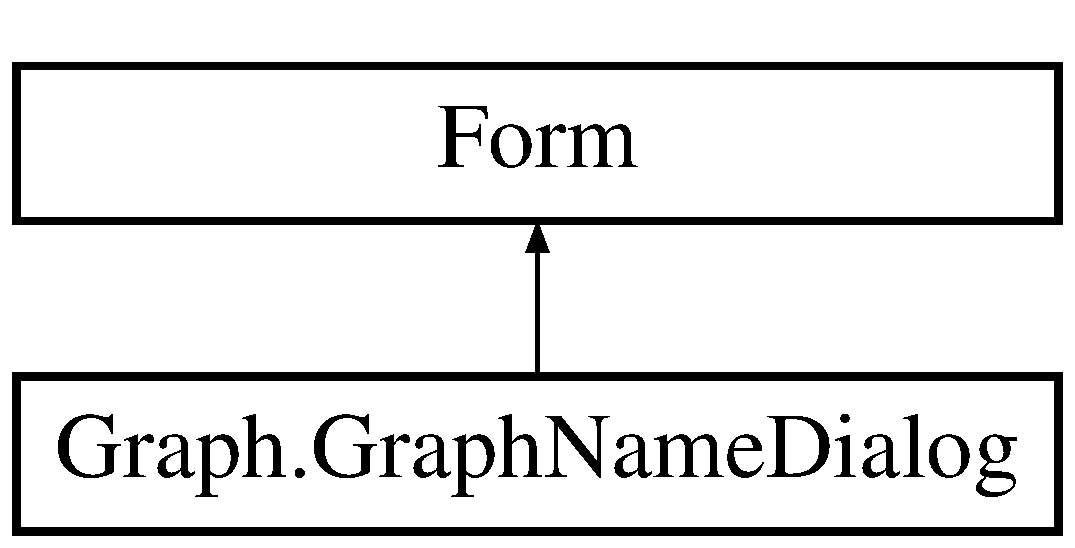
\includegraphics[height=2.000000cm]{class_graph_1_1_graph_name_dialog}
\end{center}
\end{figure}
\subsection*{Public Member Functions}
\begin{DoxyCompactItemize}
\item 
\mbox{\Hypertarget{class_graph_1_1_graph_name_dialog_ab84715b9cbe7bbf5a923739f80180a94}\label{class_graph_1_1_graph_name_dialog_ab84715b9cbe7bbf5a923739f80180a94}} 
{\bfseries Graph\+Name\+Dialog} (string name)
\end{DoxyCompactItemize}
\subsection*{Protected Member Functions}
\begin{DoxyCompactItemize}
\item 
override void \hyperlink{class_graph_1_1_graph_name_dialog_a81b7a2704a245cf0cf74675f7bd01957}{Dispose} (bool disposing)
\begin{DoxyCompactList}\small\item\em Clean up any resources being used. \end{DoxyCompactList}\end{DoxyCompactItemize}
\subsection*{Properties}
\begin{DoxyCompactItemize}
\item 
\mbox{\Hypertarget{class_graph_1_1_graph_name_dialog_a1b955082f51e862fded585e8d87c223e}\label{class_graph_1_1_graph_name_dialog_a1b955082f51e862fded585e8d87c223e}} 
new string {\bfseries Name}\hspace{0.3cm}{\ttfamily  \mbox{[}get\mbox{]}}
\end{DoxyCompactItemize}


\subsection{Member Function Documentation}
\mbox{\Hypertarget{class_graph_1_1_graph_name_dialog_a81b7a2704a245cf0cf74675f7bd01957}\label{class_graph_1_1_graph_name_dialog_a81b7a2704a245cf0cf74675f7bd01957}} 
\index{Graph\+::\+Graph\+Name\+Dialog@{Graph\+::\+Graph\+Name\+Dialog}!Dispose@{Dispose}}
\index{Dispose@{Dispose}!Graph\+::\+Graph\+Name\+Dialog@{Graph\+::\+Graph\+Name\+Dialog}}
\subsubsection{\texorpdfstring{Dispose()}{Dispose()}}
{\footnotesize\ttfamily override void Graph.\+Graph\+Name\+Dialog.\+Dispose (\begin{DoxyParamCaption}\item[{bool}]{disposing }\end{DoxyParamCaption})\hspace{0.3cm}{\ttfamily [protected]}}



Clean up any resources being used. 


\begin{DoxyParams}{Parameters}
{\em disposing} & true if managed resources should be disposed; otherwise, false.\\
\hline
\end{DoxyParams}


The documentation for this class was generated from the following files\+:\begin{DoxyCompactItemize}
\item 
C\+:/\+Users/aless/\+One\+Drive/\+Documenti/\+Visual Studio 2017/\+Projects/\+Graph/\+Graph/Graph\+Name\+Dialog.\+cs\item 
C\+:/\+Users/aless/\+One\+Drive/\+Documenti/\+Visual Studio 2017/\+Projects/\+Graph/\+Graph/Graph\+Name\+Dialog.\+Designer.\+cs\end{DoxyCompactItemize}

\hypertarget{class_graph_1_1_main_window}{}\section{Graph.\+Main\+Window Class Reference}
\label{class_graph_1_1_main_window}\index{Graph.\+Main\+Window@{Graph.\+Main\+Window}}


Main Window for the application  


Inheritance diagram for Graph.\+Main\+Window\+:\begin{figure}[H]
\begin{center}
\leavevmode
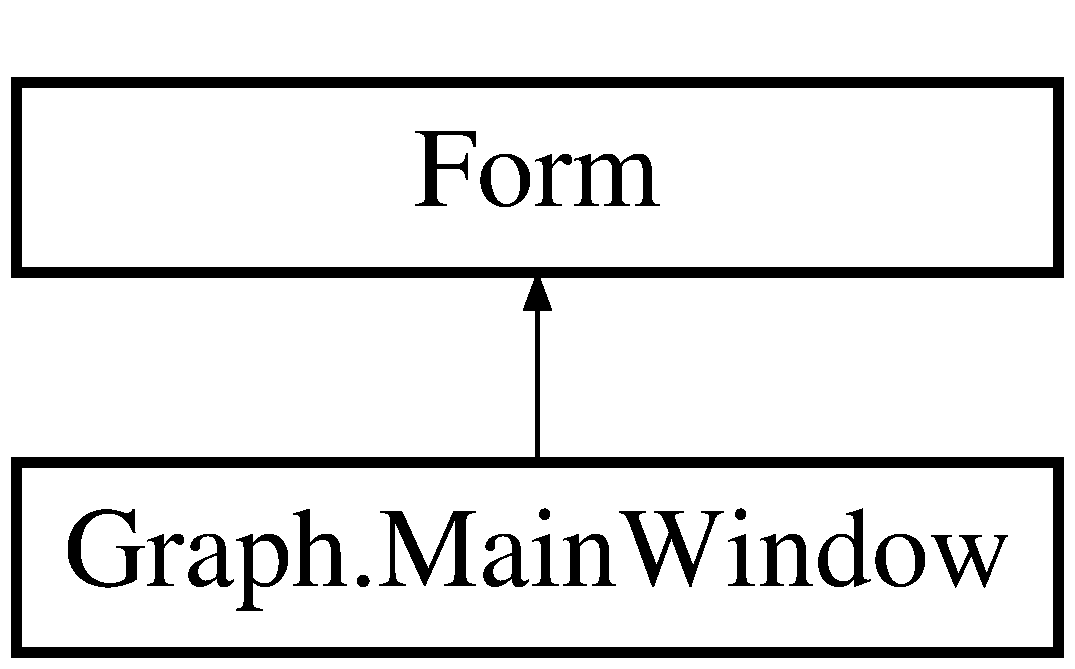
\includegraphics[height=2.000000cm]{class_graph_1_1_main_window}
\end{center}
\end{figure}
\subsection*{Public Member Functions}
\begin{DoxyCompactItemize}
\item 
\hyperlink{class_graph_1_1_main_window_a4e5941eebddebf1918da2106ee3d7e22}{Main\+Window} ()
\begin{DoxyCompactList}\small\item\em Construct a new \hyperlink{class_graph_1_1_main_window}{Main\+Window} \end{DoxyCompactList}\item 
void \hyperlink{class_graph_1_1_main_window_a6aec2f5a712c2581c9cd08878251af3f}{Update\+Graphics} ()
\begin{DoxyCompactList}\small\item\em Updates the graph view \end{DoxyCompactList}\end{DoxyCompactItemize}
\subsection*{Protected Member Functions}
\begin{DoxyCompactItemize}
\item 
override void \hyperlink{class_graph_1_1_main_window_a79dbc89bca54467324ea936e580f380e}{Dispose} (bool disposing)
\begin{DoxyCompactList}\small\item\em Clean up any resources being used. \end{DoxyCompactList}\end{DoxyCompactItemize}


\subsection{Detailed Description}
Main Window for the application 



\subsection{Constructor \& Destructor Documentation}
\mbox{\Hypertarget{class_graph_1_1_main_window_a4e5941eebddebf1918da2106ee3d7e22}\label{class_graph_1_1_main_window_a4e5941eebddebf1918da2106ee3d7e22}} 
\index{Graph\+::\+Main\+Window@{Graph\+::\+Main\+Window}!Main\+Window@{Main\+Window}}
\index{Main\+Window@{Main\+Window}!Graph\+::\+Main\+Window@{Graph\+::\+Main\+Window}}
\subsubsection{\texorpdfstring{Main\+Window()}{MainWindow()}}
{\footnotesize\ttfamily Graph.\+Main\+Window.\+Main\+Window (\begin{DoxyParamCaption}{ }\end{DoxyParamCaption})}



Construct a new \hyperlink{class_graph_1_1_main_window}{Main\+Window} 



\subsection{Member Function Documentation}
\mbox{\Hypertarget{class_graph_1_1_main_window_a79dbc89bca54467324ea936e580f380e}\label{class_graph_1_1_main_window_a79dbc89bca54467324ea936e580f380e}} 
\index{Graph\+::\+Main\+Window@{Graph\+::\+Main\+Window}!Dispose@{Dispose}}
\index{Dispose@{Dispose}!Graph\+::\+Main\+Window@{Graph\+::\+Main\+Window}}
\subsubsection{\texorpdfstring{Dispose()}{Dispose()}}
{\footnotesize\ttfamily override void Graph.\+Main\+Window.\+Dispose (\begin{DoxyParamCaption}\item[{bool}]{disposing }\end{DoxyParamCaption})\hspace{0.3cm}{\ttfamily [protected]}}



Clean up any resources being used. 


\begin{DoxyParams}{Parameters}
{\em disposing} & true if managed resources should be disposed; otherwise, false.\\
\hline
\end{DoxyParams}
\mbox{\Hypertarget{class_graph_1_1_main_window_a6aec2f5a712c2581c9cd08878251af3f}\label{class_graph_1_1_main_window_a6aec2f5a712c2581c9cd08878251af3f}} 
\index{Graph\+::\+Main\+Window@{Graph\+::\+Main\+Window}!Update\+Graphics@{Update\+Graphics}}
\index{Update\+Graphics@{Update\+Graphics}!Graph\+::\+Main\+Window@{Graph\+::\+Main\+Window}}
\subsubsection{\texorpdfstring{Update\+Graphics()}{UpdateGraphics()}}
{\footnotesize\ttfamily void Graph.\+Main\+Window.\+Update\+Graphics (\begin{DoxyParamCaption}{ }\end{DoxyParamCaption})}



Updates the graph view 



The documentation for this class was generated from the following files\+:\begin{DoxyCompactItemize}
\item 
C\+:/\+Users/aless/\+One\+Drive/\+Documenti/\+Visual Studio 2017/\+Projects/\+Graph/\+Graph/Main\+Window.\+cs\item 
C\+:/\+Users/aless/\+One\+Drive/\+Documenti/\+Visual Studio 2017/\+Projects/\+Graph/\+Graph/Main\+Window.\+Designer.\+cs\end{DoxyCompactItemize}

\hypertarget{class_graph_1_1_new_vertex_dialog}{}\section{Graph.\+New\+Vertex\+Dialog Class Reference}
\label{class_graph_1_1_new_vertex_dialog}\index{Graph.\+New\+Vertex\+Dialog@{Graph.\+New\+Vertex\+Dialog}}
Inheritance diagram for Graph.\+New\+Vertex\+Dialog\+:\begin{figure}[H]
\begin{center}
\leavevmode
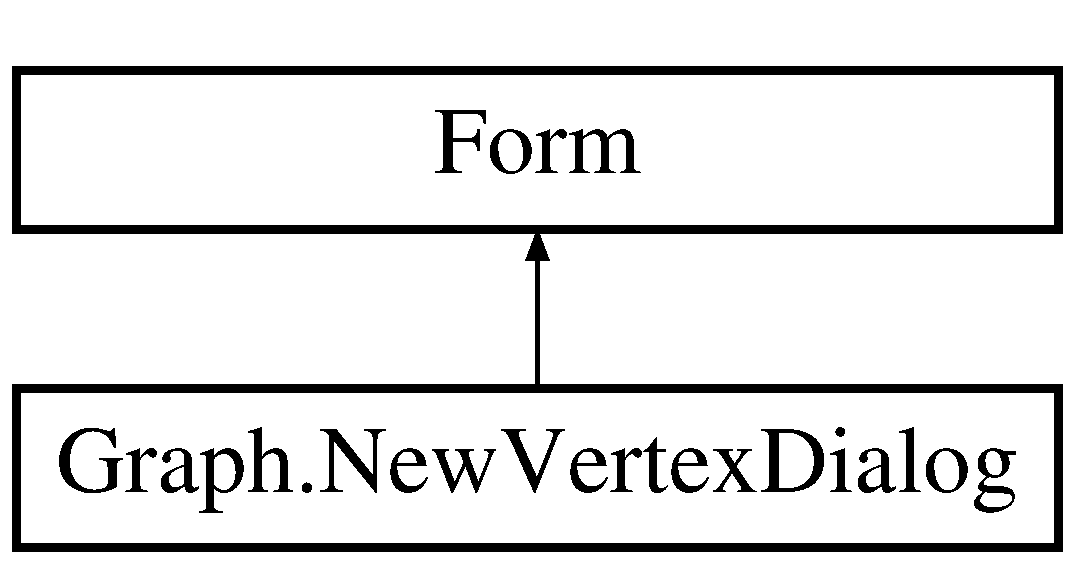
\includegraphics[height=2.000000cm]{class_graph_1_1_new_vertex_dialog}
\end{center}
\end{figure}
\subsection*{Protected Member Functions}
\begin{DoxyCompactItemize}
\item 
override void \hyperlink{class_graph_1_1_new_vertex_dialog_a92dfc769811c7d1832117f8c7054b564}{Dispose} (bool disposing)
\begin{DoxyCompactList}\small\item\em Clean up any resources being used. \end{DoxyCompactList}\end{DoxyCompactItemize}
\subsection*{Properties}
\begin{DoxyCompactItemize}
\item 
\mbox{\Hypertarget{class_graph_1_1_new_vertex_dialog_ae24171e3e7f7b248dd9e2efeb41f7f7c}\label{class_graph_1_1_new_vertex_dialog_ae24171e3e7f7b248dd9e2efeb41f7f7c}} 
new string {\bfseries Name}\hspace{0.3cm}{\ttfamily  \mbox{[}get\mbox{]}}
\end{DoxyCompactItemize}


\subsection{Member Function Documentation}
\mbox{\Hypertarget{class_graph_1_1_new_vertex_dialog_a92dfc769811c7d1832117f8c7054b564}\label{class_graph_1_1_new_vertex_dialog_a92dfc769811c7d1832117f8c7054b564}} 
\index{Graph\+::\+New\+Vertex\+Dialog@{Graph\+::\+New\+Vertex\+Dialog}!Dispose@{Dispose}}
\index{Dispose@{Dispose}!Graph\+::\+New\+Vertex\+Dialog@{Graph\+::\+New\+Vertex\+Dialog}}
\subsubsection{\texorpdfstring{Dispose()}{Dispose()}}
{\footnotesize\ttfamily override void Graph.\+New\+Vertex\+Dialog.\+Dispose (\begin{DoxyParamCaption}\item[{bool}]{disposing }\end{DoxyParamCaption})\hspace{0.3cm}{\ttfamily [protected]}}



Clean up any resources being used. 


\begin{DoxyParams}{Parameters}
{\em disposing} & true if managed resources should be disposed; otherwise, false.\\
\hline
\end{DoxyParams}


The documentation for this class was generated from the following files\+:\begin{DoxyCompactItemize}
\item 
C\+:/\+Users/aless/\+One\+Drive/\+Documenti/\+Visual Studio 2017/\+Projects/\+Graph/\+Graph/New\+Vertex\+Dialog.\+cs\item 
C\+:/\+Users/aless/\+One\+Drive/\+Documenti/\+Visual Studio 2017/\+Projects/\+Graph/\+Graph/New\+Vertex\+Dialog.\+Designer.\+cs\end{DoxyCompactItemize}

\hypertarget{class_graph_1_1_algorithm_1_1_no_such_path_exception}{}\section{Graph.\+Algorithm.\+No\+Such\+Path\+Exception Class Reference}
\label{class_graph_1_1_algorithm_1_1_no_such_path_exception}\index{Graph.\+Algorithm.\+No\+Such\+Path\+Exception@{Graph.\+Algorithm.\+No\+Such\+Path\+Exception}}


An exception that is thrown when the path from A to B doesn\textquotesingle{}t exist  


Inheritance diagram for Graph.\+Algorithm.\+No\+Such\+Path\+Exception\+:\begin{figure}[H]
\begin{center}
\leavevmode
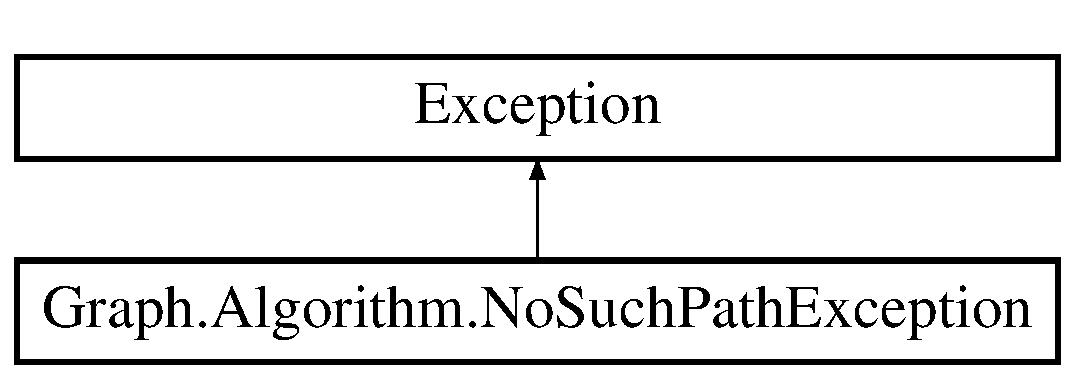
\includegraphics[height=2.000000cm]{class_graph_1_1_algorithm_1_1_no_such_path_exception}
\end{center}
\end{figure}


\subsection{Detailed Description}
An exception that is thrown when the path from A to B doesn\textquotesingle{}t exist 



The documentation for this class was generated from the following file\+:\begin{DoxyCompactItemize}
\item 
C\+:/\+Users/aless/\+One\+Drive/\+Documenti/\+Visual Studio 2017/\+Projects/\+Graph/\+Graph/Algorithm.\+cs\end{DoxyCompactItemize}

\hypertarget{class_graph_1_1_vertex}{}\section{Graph.\+Vertex Class Reference}
\label{class_graph_1_1_vertex}\index{Graph.\+Vertex@{Graph.\+Vertex}}


A class that represents a vertex in a graph  


\subsection*{Public Member Functions}
\begin{DoxyCompactItemize}
\item 
\hyperlink{class_graph_1_1_vertex_a65e1270ac657e57f3b4ed62434bc1a14}{Vertex} (string name)
\begin{DoxyCompactList}\small\item\em Constructor of a vertex \end{DoxyCompactList}\item 
\hyperlink{class_graph_1_1_vertex_ab0e830faa738a8c022a7c24b0f86ab9c}{Vertex} (string name, int x, int y)
\begin{DoxyCompactList}\small\item\em Construct a new vertex on the given position \end{DoxyCompactList}\item 
void \hyperlink{class_graph_1_1_vertex_ac356de9ce319961880faa5f7390435fa}{Add\+Edge} (\hyperlink{class_graph_1_1_vertex}{Vertex} to, int weight)
\begin{DoxyCompactList}\small\item\em Adds an edge from this vertex \end{DoxyCompactList}\item 
void \hyperlink{class_graph_1_1_vertex_a634f39ee548903000dd1b8c702351fe8}{Remove\+Edge} (\hyperlink{class_graph_1_1_vertex}{Vertex} to)
\begin{DoxyCompactList}\small\item\em Removes an edge \end{DoxyCompactList}\item 
I\+Enumerator \hyperlink{class_graph_1_1_vertex_a74a735028c6c203ddc42f63033dcb66a}{Get\+Enumerator} ()
\begin{DoxyCompactList}\small\item\em Iterates on node neighbors \end{DoxyCompactList}\item 
override string \hyperlink{class_graph_1_1_vertex_a235f3019b6b480a8bf4c8116a5d30bf4}{To\+String} ()
\begin{DoxyCompactList}\small\item\em Returns string rappresentation of the vertex, in practice its name \end{DoxyCompactList}\item 
int \hyperlink{class_graph_1_1_vertex_aa96f873cf862f818c345a5d97c3b62c1}{Get\+Weight\+To} (\hyperlink{class_graph_1_1_vertex}{Vertex} to)
\begin{DoxyCompactList}\small\item\em Gets the edge weight from this vertex to the one specified \end{DoxyCompactList}\end{DoxyCompactItemize}
\subsection*{Public Attributes}
\begin{DoxyCompactItemize}
\item 
int \hyperlink{class_graph_1_1_vertex_ab165fd05985d7ab12341f97abcde9e79}{Exit\+Grade} =$>$ Edges.\+Count
\begin{DoxyCompactList}\small\item\em Returns the exit grade of the vertex \end{DoxyCompactList}\item 
int \hyperlink{class_graph_1_1_vertex_a120c6d309edf2487e4d7d8463f586dc4}{Grade} =$>$ \hyperlink{class_graph_1_1_vertex_ab165fd05985d7ab12341f97abcde9e79}{Exit\+Grade} + \hyperlink{class_graph_1_1_vertex_a63c478ac5624dcd7d424212e1b4fa923}{Enter\+Grade}
\begin{DoxyCompactList}\small\item\em Totale grade of the vertex \end{DoxyCompactList}\end{DoxyCompactItemize}
\subsection*{Properties}
\begin{DoxyCompactItemize}
\item 
Dictionary$<$ \hyperlink{class_graph_1_1_vertex}{Vertex}, int $>$ \hyperlink{class_graph_1_1_vertex_a494371449797e8a7d9c26d6a49922f42}{Edges}\hspace{0.3cm}{\ttfamily  \mbox{[}get\mbox{]}}
\begin{DoxyCompactList}\small\item\em \hyperlink{class_graph_1_1_edge}{Edge} dictionary, every \hyperlink{class_graph_1_1_vertex}{Vertex} that the edge connects to has associated its weight \end{DoxyCompactList}\item 
string \hyperlink{class_graph_1_1_vertex_aa0cafbcfdc99942d4b3942abf6d21894}{Name} = new Dictionary$<$\hyperlink{class_graph_1_1_vertex}{Vertex}, int$>$()\hspace{0.3cm}{\ttfamily  \mbox{[}get\mbox{]}}
\begin{DoxyCompactList}\small\item\em Name of the vertex \end{DoxyCompactList}\item 
int \hyperlink{class_graph_1_1_vertex_af2284092cc5f24be9656338f4e2fe80f}{X}\hspace{0.3cm}{\ttfamily  \mbox{[}get, set\mbox{]}}
\begin{DoxyCompactList}\small\item\em X position of the vertex \end{DoxyCompactList}\item 
int \hyperlink{class_graph_1_1_vertex_a7166c79bcdc4d67314cd16b456a24dd2}{Y}\hspace{0.3cm}{\ttfamily  \mbox{[}get, set\mbox{]}}
\begin{DoxyCompactList}\small\item\em Y position of the vertex \end{DoxyCompactList}\item 
bool \hyperlink{class_graph_1_1_vertex_a06cc9a5a43a8a9fb1715b19a8877ed01}{Color}\hspace{0.3cm}{\ttfamily  \mbox{[}get, set\mbox{]}}
\begin{DoxyCompactList}\small\item\em Color of the vertex -\/ true = red, false = black \end{DoxyCompactList}\item 
int \hyperlink{class_graph_1_1_vertex_a63c478ac5624dcd7d424212e1b4fa923}{Enter\+Grade}\hspace{0.3cm}{\ttfamily  \mbox{[}get\mbox{]}}
\begin{DoxyCompactList}\small\item\em Enter grade of the vertex \end{DoxyCompactList}\end{DoxyCompactItemize}


\subsection{Detailed Description}
A class that represents a vertex in a graph 



\subsection{Constructor \& Destructor Documentation}
\mbox{\Hypertarget{class_graph_1_1_vertex_a65e1270ac657e57f3b4ed62434bc1a14}\label{class_graph_1_1_vertex_a65e1270ac657e57f3b4ed62434bc1a14}} 
\index{Graph\+::\+Vertex@{Graph\+::\+Vertex}!Vertex@{Vertex}}
\index{Vertex@{Vertex}!Graph\+::\+Vertex@{Graph\+::\+Vertex}}
\subsubsection{\texorpdfstring{Vertex()}{Vertex()}\hspace{0.1cm}{\footnotesize\ttfamily [1/2]}}
{\footnotesize\ttfamily Graph.\+Vertex.\+Vertex (\begin{DoxyParamCaption}\item[{string}]{name }\end{DoxyParamCaption})}



Constructor of a vertex 


\begin{DoxyParams}{Parameters}
{\em name} & The name of the vertex\\
\hline
\end{DoxyParams}
\mbox{\Hypertarget{class_graph_1_1_vertex_ab0e830faa738a8c022a7c24b0f86ab9c}\label{class_graph_1_1_vertex_ab0e830faa738a8c022a7c24b0f86ab9c}} 
\index{Graph\+::\+Vertex@{Graph\+::\+Vertex}!Vertex@{Vertex}}
\index{Vertex@{Vertex}!Graph\+::\+Vertex@{Graph\+::\+Vertex}}
\subsubsection{\texorpdfstring{Vertex()}{Vertex()}\hspace{0.1cm}{\footnotesize\ttfamily [2/2]}}
{\footnotesize\ttfamily Graph.\+Vertex.\+Vertex (\begin{DoxyParamCaption}\item[{string}]{name,  }\item[{int}]{x,  }\item[{int}]{y }\end{DoxyParamCaption})}



Construct a new vertex on the given position 


\begin{DoxyParams}{Parameters}
{\em name} & name of the vertex\\
\hline
{\em x} & x coordinate\\
\hline
{\em y} & y coordinate\\
\hline
\end{DoxyParams}


\subsection{Member Function Documentation}
\mbox{\Hypertarget{class_graph_1_1_vertex_ac356de9ce319961880faa5f7390435fa}\label{class_graph_1_1_vertex_ac356de9ce319961880faa5f7390435fa}} 
\index{Graph\+::\+Vertex@{Graph\+::\+Vertex}!Add\+Edge@{Add\+Edge}}
\index{Add\+Edge@{Add\+Edge}!Graph\+::\+Vertex@{Graph\+::\+Vertex}}
\subsubsection{\texorpdfstring{Add\+Edge()}{AddEdge()}}
{\footnotesize\ttfamily void Graph.\+Vertex.\+Add\+Edge (\begin{DoxyParamCaption}\item[{\hyperlink{class_graph_1_1_vertex}{Vertex}}]{to,  }\item[{int}]{weight }\end{DoxyParamCaption})}



Adds an edge from this vertex 


\begin{DoxyParams}{Parameters}
{\em to} & vertex to connect\\
\hline
{\em weight} & weight of the edge\\
\hline
\end{DoxyParams}
\mbox{\Hypertarget{class_graph_1_1_vertex_a74a735028c6c203ddc42f63033dcb66a}\label{class_graph_1_1_vertex_a74a735028c6c203ddc42f63033dcb66a}} 
\index{Graph\+::\+Vertex@{Graph\+::\+Vertex}!Get\+Enumerator@{Get\+Enumerator}}
\index{Get\+Enumerator@{Get\+Enumerator}!Graph\+::\+Vertex@{Graph\+::\+Vertex}}
\subsubsection{\texorpdfstring{Get\+Enumerator()}{GetEnumerator()}}
{\footnotesize\ttfamily I\+Enumerator Graph.\+Vertex.\+Get\+Enumerator (\begin{DoxyParamCaption}{ }\end{DoxyParamCaption})}



Iterates on node neighbors 

\begin{DoxyReturn}{Returns}
Neighbors iterator
\end{DoxyReturn}
\mbox{\Hypertarget{class_graph_1_1_vertex_aa96f873cf862f818c345a5d97c3b62c1}\label{class_graph_1_1_vertex_aa96f873cf862f818c345a5d97c3b62c1}} 
\index{Graph\+::\+Vertex@{Graph\+::\+Vertex}!Get\+Weight\+To@{Get\+Weight\+To}}
\index{Get\+Weight\+To@{Get\+Weight\+To}!Graph\+::\+Vertex@{Graph\+::\+Vertex}}
\subsubsection{\texorpdfstring{Get\+Weight\+To()}{GetWeightTo()}}
{\footnotesize\ttfamily int Graph.\+Vertex.\+Get\+Weight\+To (\begin{DoxyParamCaption}\item[{\hyperlink{class_graph_1_1_vertex}{Vertex}}]{to }\end{DoxyParamCaption})}



Gets the edge weight from this vertex to the one specified 


\begin{DoxyParams}{Parameters}
{\em to} & vertex to go to\\
\hline
\end{DoxyParams}
\begin{DoxyReturn}{Returns}
the weight of the edge between this vertex and the one specified
\end{DoxyReturn}
\mbox{\Hypertarget{class_graph_1_1_vertex_a634f39ee548903000dd1b8c702351fe8}\label{class_graph_1_1_vertex_a634f39ee548903000dd1b8c702351fe8}} 
\index{Graph\+::\+Vertex@{Graph\+::\+Vertex}!Remove\+Edge@{Remove\+Edge}}
\index{Remove\+Edge@{Remove\+Edge}!Graph\+::\+Vertex@{Graph\+::\+Vertex}}
\subsubsection{\texorpdfstring{Remove\+Edge()}{RemoveEdge()}}
{\footnotesize\ttfamily void Graph.\+Vertex.\+Remove\+Edge (\begin{DoxyParamCaption}\item[{\hyperlink{class_graph_1_1_vertex}{Vertex}}]{to }\end{DoxyParamCaption})}



Removes an edge 


\begin{DoxyParams}{Parameters}
{\em to} & destination vertex to remove\\
\hline
\end{DoxyParams}
\mbox{\Hypertarget{class_graph_1_1_vertex_a235f3019b6b480a8bf4c8116a5d30bf4}\label{class_graph_1_1_vertex_a235f3019b6b480a8bf4c8116a5d30bf4}} 
\index{Graph\+::\+Vertex@{Graph\+::\+Vertex}!To\+String@{To\+String}}
\index{To\+String@{To\+String}!Graph\+::\+Vertex@{Graph\+::\+Vertex}}
\subsubsection{\texorpdfstring{To\+String()}{ToString()}}
{\footnotesize\ttfamily override string Graph.\+Vertex.\+To\+String (\begin{DoxyParamCaption}{ }\end{DoxyParamCaption})}



Returns string rappresentation of the vertex, in practice its name 

\begin{DoxyReturn}{Returns}
string rappresentation of the vertex
\end{DoxyReturn}


\subsection{Member Data Documentation}
\mbox{\Hypertarget{class_graph_1_1_vertex_ab165fd05985d7ab12341f97abcde9e79}\label{class_graph_1_1_vertex_ab165fd05985d7ab12341f97abcde9e79}} 
\index{Graph\+::\+Vertex@{Graph\+::\+Vertex}!Exit\+Grade@{Exit\+Grade}}
\index{Exit\+Grade@{Exit\+Grade}!Graph\+::\+Vertex@{Graph\+::\+Vertex}}
\subsubsection{\texorpdfstring{Exit\+Grade}{ExitGrade}}
{\footnotesize\ttfamily int Graph.\+Vertex.\+Exit\+Grade =$>$ Edges.\+Count}



Returns the exit grade of the vertex 

\mbox{\Hypertarget{class_graph_1_1_vertex_a120c6d309edf2487e4d7d8463f586dc4}\label{class_graph_1_1_vertex_a120c6d309edf2487e4d7d8463f586dc4}} 
\index{Graph\+::\+Vertex@{Graph\+::\+Vertex}!Grade@{Grade}}
\index{Grade@{Grade}!Graph\+::\+Vertex@{Graph\+::\+Vertex}}
\subsubsection{\texorpdfstring{Grade}{Grade}}
{\footnotesize\ttfamily int Graph.\+Vertex.\+Grade =$>$ \hyperlink{class_graph_1_1_vertex_ab165fd05985d7ab12341f97abcde9e79}{Exit\+Grade} + \hyperlink{class_graph_1_1_vertex_a63c478ac5624dcd7d424212e1b4fa923}{Enter\+Grade}}



Totale grade of the vertex 



\subsection{Property Documentation}
\mbox{\Hypertarget{class_graph_1_1_vertex_a06cc9a5a43a8a9fb1715b19a8877ed01}\label{class_graph_1_1_vertex_a06cc9a5a43a8a9fb1715b19a8877ed01}} 
\index{Graph\+::\+Vertex@{Graph\+::\+Vertex}!Color@{Color}}
\index{Color@{Color}!Graph\+::\+Vertex@{Graph\+::\+Vertex}}
\subsubsection{\texorpdfstring{Color}{Color}}
{\footnotesize\ttfamily bool Graph.\+Vertex.\+Color\hspace{0.3cm}{\ttfamily [get]}, {\ttfamily [set]}}



Color of the vertex -\/ true = red, false = black 

\mbox{\Hypertarget{class_graph_1_1_vertex_a494371449797e8a7d9c26d6a49922f42}\label{class_graph_1_1_vertex_a494371449797e8a7d9c26d6a49922f42}} 
\index{Graph\+::\+Vertex@{Graph\+::\+Vertex}!Edges@{Edges}}
\index{Edges@{Edges}!Graph\+::\+Vertex@{Graph\+::\+Vertex}}
\subsubsection{\texorpdfstring{Edges}{Edges}}
{\footnotesize\ttfamily Dictionary$<$\hyperlink{class_graph_1_1_vertex}{Vertex}, int$>$ Graph.\+Vertex.\+Edges\hspace{0.3cm}{\ttfamily [get]}}



\hyperlink{class_graph_1_1_edge}{Edge} dictionary, every \hyperlink{class_graph_1_1_vertex}{Vertex} that the edge connects to has associated its weight 

\mbox{\Hypertarget{class_graph_1_1_vertex_a63c478ac5624dcd7d424212e1b4fa923}\label{class_graph_1_1_vertex_a63c478ac5624dcd7d424212e1b4fa923}} 
\index{Graph\+::\+Vertex@{Graph\+::\+Vertex}!Enter\+Grade@{Enter\+Grade}}
\index{Enter\+Grade@{Enter\+Grade}!Graph\+::\+Vertex@{Graph\+::\+Vertex}}
\subsubsection{\texorpdfstring{Enter\+Grade}{EnterGrade}}
{\footnotesize\ttfamily int Graph.\+Vertex.\+Enter\+Grade\hspace{0.3cm}{\ttfamily [get]}}



Enter grade of the vertex 

\mbox{\Hypertarget{class_graph_1_1_vertex_aa0cafbcfdc99942d4b3942abf6d21894}\label{class_graph_1_1_vertex_aa0cafbcfdc99942d4b3942abf6d21894}} 
\index{Graph\+::\+Vertex@{Graph\+::\+Vertex}!Name@{Name}}
\index{Name@{Name}!Graph\+::\+Vertex@{Graph\+::\+Vertex}}
\subsubsection{\texorpdfstring{Name}{Name}}
{\footnotesize\ttfamily string Graph.\+Vertex.\+Name = new Dictionary$<$\hyperlink{class_graph_1_1_vertex}{Vertex}, int$>$()\hspace{0.3cm}{\ttfamily [get]}}



Name of the vertex 

\mbox{\Hypertarget{class_graph_1_1_vertex_af2284092cc5f24be9656338f4e2fe80f}\label{class_graph_1_1_vertex_af2284092cc5f24be9656338f4e2fe80f}} 
\index{Graph\+::\+Vertex@{Graph\+::\+Vertex}!X@{X}}
\index{X@{X}!Graph\+::\+Vertex@{Graph\+::\+Vertex}}
\subsubsection{\texorpdfstring{X}{X}}
{\footnotesize\ttfamily int Graph.\+Vertex.\+X\hspace{0.3cm}{\ttfamily [get]}, {\ttfamily [set]}}



X position of the vertex 

\mbox{\Hypertarget{class_graph_1_1_vertex_a7166c79bcdc4d67314cd16b456a24dd2}\label{class_graph_1_1_vertex_a7166c79bcdc4d67314cd16b456a24dd2}} 
\index{Graph\+::\+Vertex@{Graph\+::\+Vertex}!Y@{Y}}
\index{Y@{Y}!Graph\+::\+Vertex@{Graph\+::\+Vertex}}
\subsubsection{\texorpdfstring{Y}{Y}}
{\footnotesize\ttfamily int Graph.\+Vertex.\+Y\hspace{0.3cm}{\ttfamily [get]}, {\ttfamily [set]}}



Y position of the vertex 



The documentation for this class was generated from the following file\+:\begin{DoxyCompactItemize}
\item 
C\+:/\+Users/aless/\+One\+Drive/\+Documenti/\+Visual Studio 2017/\+Projects/\+Graph/\+Graph/Vertex.\+cs\end{DoxyCompactItemize}

%--- End generated contents ---

% Index
\backmatter
\newpage
\phantomsection
\clearemptydoublepage
\addcontentsline{toc}{chapter}{Index}
\printindex

\end{document}
